\documentclass[twoside,a4paper]{report}

\usepackage[pdftex]{graphicx}
\usepackage{textcomp}
\usepackage{titlesec}
\titleformat{\chapter}[display]
{\normalfont\bfseries}{}{0pt}{\huge}
\usepackage{lipsum}
\usepackage{wrapfig}
\usepackage{adjustbox}
\usepackage[utf8]{inputenc}
\usepackage[polish]{babel}
\usepackage[T1]{fontenc}
\usepackage[fit]{truncate}
\usepackage{array}
\usepackage{makecell}
\usepackage{float}
\usepackage{anysize}
\usepackage{enumitem}
\usepackage[font=small,labelfont=bf]{caption}
\usepackage{url}
\usepackage{hyperref}
\usepackage{csquotes}
\usepackage[
sorting=none
]{biblatex}
\emergencystretch=1em
\addbibresource{bibliografia.bib}
\usepackage{listings}
\renewcommand{\ttdefault}{pcr}
\usepackage{fancyhdr}
\usepackage{multirow}
\usepackage{tabularx}
\usepackage{indentfirst}
\usepackage{gensymb}
\newcolumntype{C}{>{\centering\arraybackslash}X}

\newcommand*{\noaddvspace}{\renewcommand*{\addvspace}[1]{}}
\addtocontents{lof}{\protect\noaddvspace}

\pagestyle{fancy}
\fancyhf{}

\graphicspath{{img}}

\renewcommand{\lstlistlistingname}{Spis listingów}

\lstdefinelanguage{JavaScript}{
    keywords={function, class, extends, return, render},
}

\lstdefinelanguage{Elm}{
    keywords={type, alias, update, case, of, init, view},
}

\lstset{
  basicstyle=\ttfamily,
  keywordstyle=\textbf,
  columns=fullflexible,
  frame=single,
  breaklines=true,
}

\renewcommand{\chaptermark}[1]{\markboth{#1}{}}
\renewcommand{\sectionmark}[1]{\markright{\thesection\ #1}}
\renewcommand{\headrulewidth}{0.5pt}
\renewcommand{\footrulewidth}{0pt}

\fancyhead[LE,RO]{\bfseries\thepage}
\fancyhead[LO]{\nouppercase{\bfseries{\truncate{.95\headwidth}{\rightmark}}}}
\fancyhead[RE]{\nouppercase{\bfseries{\truncate{.95\headwidth}{\leftmark}}}}

\linespread{1.5}

\parskip0.05in

\marginsize{3.5cm}{2.5cm}{2.5cm}{2.5cm}
\fancyhfoffset[E,O]{0pt}

% ---------------------------------------------------------------------------------------------------------------------

\begin{document}

% allows useg @ as a @ not as special character
% required for macro redefinition
\makeatletter

% parameters definition
% they cannot conflict with other
% like bibteh attributes etc.
\def\tytul#1{\def\@tytul{#1}}
\def\promotor#1{\def\@promotor{#1}}
\def\miasto#1{\def\@miasto{#1}}
\def\studies#1{\def\@studies{#1}}
\def\descr#1{\def\@descr{#1}}
\def\indeks#1{\def\@indeks{#1}}
\def\dept#1{\def\@dept{#1}}
\def\spec#1{\def\@spec{#1}}

\def\maketitle{
    %removal of header
    \keepXColumns
    \thispagestyle{empty}%
    \begin{center}
        \begin{tabularx}{\textwidth}{CcC}
            \multirow{4}{*}{
\includegraphics[height=2.35cm]{img/logo_pg.png}}
          & \textsc{\textbf{Politechnika Gdańska}} &
          \multirow{4}{*}{
\includegraphics[height=2.35cm]{img/logo_eti.png}}
       \\ & & \\
          & \textsc{\textbf{Wydział Elektroniki, }}& \\
          & \textsc{\textbf{Telekomunikacji i Informatyki }}& \\
        \end{tabularx}
    \end{center}
    \begin{center}
        \begin{tabularx}{\textwidth}{XX}
            \textbf{Katedra:} & \@dept\\
                              &\\
            \textbf{Imię i nazwisko dyplomanta:} & \@author\\
                                                 &\\
            \textbf{Nr albumu:} & \@indeks\\
                                &\\
            \textbf{Forma i poziom studiów:} & \@studies\\
                                             &\\
            \textbf{Kierunek studiów:} & Informatyka\\
                                       &\\
            \textbf{Specjalność:} & \@spec
        \end{tabularx}
    \end{center}
    \begin{center}
        \Large{\textbf{Praca dyplomowa magisterska}}
    \end{center}
    \vspace{1cm}
    \begin{tabular}{l}
        \textbf{Temat pracy:} \\ \@tytul\\
        \\
        \textbf{Title of thesis:} \\ \@title\\
        \\
        \textbf{Opiekun pracy:} \\ \@promotor\\
        \\
        \textbf{Data ostatecznego zatwierdzenia raportu podobieństw w JSA:} TBA
    \end{tabular}
    \vspace*{\stretch{6}}
    \begin{center}
        \@miasto, \@date
    \end{center}

}

%restore @ sign
\makeatother

\cleardoublepage


\tytul{Wykorzystanie języka Elm do tworzenia aplikacji frontendowych.}
\title{Programming the front-end applications with Elm language.}
\author{Marcin Jurczak}
\date{2022}
\miasto{Gdańsk}
\promotor{dr\ inż.\ Krzysztof Manuszewski}
\studies{Stacjonarne jednolite studia magisterskie}
\indeks{171641}
\dept{Algorytmów i Modelowania Systemów}
\spec{Algorytmów i Technologii Internetowych}

\maketitle

% ---------------------------------------------------------------------------------------------------------------------

\chapter*{Streszczenie}
\noindent
Celem niniejszej pracy magisterskiej było stworzenie frontend'owej aplikacji internetowej z wykorzystaniem funkcyjnego języka Elm, porównanie tejże technologii z istniejącymi, bardziej powszechnymi rozwiązaniami tego typu, a także przygotowanie instrukcji laboratoryjnej, która mogłaby zostać wykorzystana w ramach zajęć \textit{,,Współczesne Aplikacje Programowania Funkcyjnego''} przeprowadzanych na Wydziale Elektroniki, Telekomunikacji i Informatyki Politechniki Gdańskiej. Wytworzona aplikacja to strona internetowa typu \textit{startpage}, czyli startowa strona przeglądarki, zawierająca najpotrzebniejsze informacje, takie jak czas, pogoda oraz odnośniki do wyszukiwarki i najczęściej odwiedzanych stron.

\textbf{Słowa kluczowe:} Elm, programowanie funkcyjne, wytwarzane aplikacji internetowych

\textbf{Dziedzina nauki i techniki: }Nauki inżynieryjne i techniczne, inżynieria informatyczna.

{\let\clearpage\relax\chapter*{Abstract}}
\noindent
The goal of this master thesis is to use the Elm language to create a frontend web application, comparing this technology to existing, more popular solutions, as well as preparing a lab instruction, which could be used at \textit{,,Modern applications of functional programming''} class at Gdańsk University of Technology’s Faculty of Electronics, Telecommunications and Informatics. The created application is a \textit{startpage}, meaning a starting page of a web browser consisting of the most useful information, such as time, weather and references to search engine and the most visited websites.

\textbf{Keywords:} Elm, functional programming, web development

\textbf{Field of Science and Technology:} Engineering and Technology, Information engineering.

% ---------------------------------------------------------------------------------------------------------------------

\tableofcontents

% ---------------------------------------------------------------------------------------------------------------------

\chapter*{Wykaz najważniejszych skrótów}
\begin{tabular}{rcl}
    \textbf{API} &---& ang.~Application Programming Interface,\\
                 &   & pol.~interfejs programowania aplikacji\\
    \textbf{CD} &---& ang.~Continuous Deployment, pol.~ciągłe wdrażanie\\
    \textbf{CI} &---& ang.~Continuous Integration, pol.~ciągła integracja\\
    \textbf{CSS} &---& ang.~Cascading Style Sheets, pol.~kaskadowe arkusze stylów\\
    \textbf{HTML} &---& ang.~Hypertext Markup Language, pol.~hipertekstowy język znaczników\\
    \textbf{HTTP} &---& ang.~Hypertext Transfer Protocol, pol.~protokół przesyłania hipertekstu\\
    \textbf{JSON} &---& ang.~JavaScript Object Notation, pol.~tekstowy format zapisu danych\\
    \textbf{SPA} &---& ang.~Single Page Application, pol.~jednostronicowa aplikacja internetowa\\
    \textbf{DOM} &---& ang.~Document Object Model, pol.~obiektowy model dokumentu\\
\end{tabular}

% ---------------------------------------------------------------------------------------------------------------------

\chapter{Wstęp i cel pracy}
\begin{wrapfigure}{r}{0.28\textwidth}
    \centering
    
\includegraphics[width=0.28\textwidth]{elm_logo.png}
    \caption*{Logo Elma}\label{fig:elm_logo}
\end{wrapfigure}
Głównym celem niniejszej pracy jest zapoznanie się z funkcyjnym językiem programowania Elm oraz stworzenie przykładowej frontendowej aplikacji internetowej.
Ponadto chciałbym przeprowadzić porównanie tej technologii z innymi, bardziej powszechnie używanymi rozwiązaniami do tworzenia aplikacji internetowych.
Ostatnim celem pracy jest przygotowanie części dydaktycznej w postaci instrukcji laboratoryjnej, która mogłaby zostać potencjalnie wykorzystana w ramach przedmiotu Współczesne Aplikacje Programowania Funkcyjnego, prowadzonego przez mojego promotora, dra inż. Krzysztofa Manuszewskiego.

W drugim rozdziale skupiam się na przedstawieniu technologii powszechnie używanych do tworzenia frontendowych aplikacji internetowych, t.j. React.js, Angular oraz Vue.js.
Prezentuję ich zalety i wady względem siebie, a także przedstawiam cechy charakterystyczne dla każdego z nich oraz co je odróżnia między sobą.

Trzeci rozdział poświęcam na wysokopoziomowe wprowadzenie do języka Elm.
Mówię o idei jaka przyświęcała autorowi podczas tworzenia tego języka, jakie są jego potencjalne zastosowania, gdzie sprawdza się najlepiej oraz przedstawiam narzędzia wspomagające tworzenie oprogramowania z użyciem tejże technologii, włączając w to dokumentację.

W czwartm rozdziale przedstawiam implementację przygotowanej aplikacji frontendowej napisanej w Elmie.
Jest to poniekąd rozwinięcie poprzedniego rozdziału, ponieważ głównym celem jest dalej zapoznanie się z Elmem, jednak tutaj uwagę skupiam na przedstawieniu konkretnych rozwiązań, jakie zostały wykorzystane do osiągniecia wybranego celu.

Piąty rozdział zawiera instrukcję laboratoryjną, w której przeprowadzam czytelnika nieposiadającego żadnego doświadczenia z Elmem przez proces tworzenia oprogramowania z wykorzystaniem tej technologii, zaczynając od przygotowania środowiska, przez podstawy języka, aż po stworzenie aplikacji frontendowej przedstawionej we wcześniejszym rozdziale.

Szósty rozdział poświęcam na omówienie zagadnień związanych z ciągłą integracją oraz ciągłym wdrażaniem, a także przedstawiam narzędzia wykorzystywane przeze mnie w tym celu podczas tworzenia omawianej aplikacji.
Pokazuję, że Elm nie stanowi przeszkody w wykorzystywaniu tych technologii i całkowicie nadaje się do użytku produkcyjnego.

Ostatni rozdział dotyczy przede wszystkim podsumowania niniejszej pracy magisterskiej.
Przedstawiam produkt dwóch semestrów moich działań oraz wyciągam wnioski na temat Elma jako języka przeznaczonego do tworzenia aplikacji frontendowych.

Na końcu dokumentu znajdują się spisy użytych rysunków i listingów, a także bibliografia, która została wykorzystana podczas pracy nad niniejszym dokumentem oraz w czasie zapoznawania się z tematem wytwarzania aplikacji internetowych z wykorzystaniem języka Elm.

% ---------------------------------------------------------------------------------------------------------------------

\chapter{Powszechne rozwiązania}
W poniższym rozdziale chciałbym przedstawić najpopularniejsze rozwiązania do tworzenia frontendowych stron internetowych, które są powszechnie stosowane zarówno przez największych gigantów technologicznych, tj. Google, Facebook, Netflix, ale także małe, dopiero wchodządzące na rynek firmy startupowe.

Według ankiety przeprowadzonej w 2021 roku przez StackOverflow~\cite{stacksurvey}, najczęściej wybieranym przez programistów frameworkiem do tworzenia stron internetowych był React.js (40,14\% odpowiedzi), a na czwartym i piątym miejscu znajdowały się odpowiednio biblioteki Angular (22,96\% odpowiedzi) oraz Vue.js (18,97\% odpowiedzi).
Są to biblioteki, na których chciałbym się skupić w poniższych podrozdziałach.
Opiszę, czym się charakteryzują, jakie są ich wady i zalety, a także co je ze sobą łączy oraz w jaki sposób są od siebie różne.

\section{React.js}
React.js~\cite{react} jest otwartoźródłową biblioteką języka programowania JavaScript, której głównym przeznaczeniem jest tworzenie interfejsów graficznych, w większości wykorzystywana jest do aplikacji typu SPA\@.
Została stworzona w 2013 roku przez ówczesnego programistę Facebook'a, Jordana Walke.
Rozwój Reacta utrzymywany jest po dzień dzisiejszy przez~,,matczyną'' firmę Meta (dawniej znaną jako Facebook), a także przez społeczność indywidualnych programistów i innych organizacji ze względu na swoją otwartoźródłową naturę.

Tworzenie oprogramowania z użyciem tej biblioteki odbywa się poprzez budowanie nowych komponentów, które za pośrednictwem metody \texttt{render()} decydują, co ma zostać wyświetlane na ekranie użytkownika.
Według dokumentacji Reacta~\cite{reactdocs}, komponenty mogą być zdefiniowane na dwa sposoby: poprzez stworzenie JavaScript'owej funkcji lub wykorzystując klasę bazującą na \texttt{React.Component}.

Przykłady wspomnianych definicji zostały przedstawione odpowiednio na listingach~\ref{lst:func_comp} oraz~\ref{lst:class_comp}, a ich funkcjonalność jest jednakowa --- wyświetlenie napisu w formie nagłówka tagu \texttt{<h1>} o treści~,,\textit{Hello, }'' + imię zawarte w zmiennej \texttt{props}.


\begin{lstlisting}[caption={Przykład funkcyjnego komponentu},label={lst:func_comp},language=JavaScript]
function Hello(props) {
  return <h1>Hello, {props.name}</h1>;
}
\end{lstlisting}
\begin{lstlisting}[caption={Przykład klasowego komponentu},label={lst:class_comp},language=JavaScript]
class Hello extends React.Component {
  render() {
    return <h1>Hello, {this.props.name}</h1>;
  }
}
\end{lstlisting}

Jedną z cech kodu tworzonego z użyciem biblioteki React jest jego deklaratywność. Aby użyć stworzonego komponentu wystarczy go zaimportować i wykorzystać za pomocą tagu, dla powyższego przykładu tagu \texttt{<Hello name="Marcin"/>}, który dodatkowo zawiera pojedynczy argument \texttt{props}, będący obiektem z danymi, w tym przypadku zawierający imię~,,Marcin''.
Dzięki temu kod pisany przy pomocy biblioteki React jest bardzo reużywalny i pozwala na wykorzystanie komponentów nawet pomiędzy odrębnymi aplikacjami.

Jedną z zalet tego rozwiązania jest jego niesamowita popularność oraz dostępność gotowych rozwiązań.
W Internecie znajduje się mnóstwo poradników i instrukcji pomagających nowym użytkownikom zapoznać się z biblioteką i stworzyć pierwsze proste projekty.
Istnieje także dostatek pomocy dla bardziej zaawansowych programistów Reacta oraz szeroka społeczność użytkowników chętnych do pomocy przy rozwiązywaniu bardziej skomplikowanych problemów.
Dostępność gotowych rozwiązań pozwala na relatywnie łatwy rozwój oprogramowania poprzez ich wykorzystanie, dla przykładu

\section{Angular}
Biblioteka Angular~\cite{angulardocs}
~\cite{angulardocs}
\section{Vue.js}
Biblioteka Vue.js~\cite{vuejsdocs}
\section{Podobieństwa i różnice}

% ---------------------------------------------------------------------------------------------------------------------

\chapter{Elm}
Elm~\cite{elmdocs} jest czysto funkcyjnym językiem programowania przeznaczonym do tworzenia graficznych interfejsów użytkownika.
Powstał w roku 2012 wraz z opublikowaniem przez Evana Czaplickiego pracy~,,Elm: Concurrent FRP for Functional GUIs''~\cite{Czaplicki2012ElmC}.
Podczas jego tworzenia nacisk został położony na użyteczność, wydajność oraz niską podatność na błędy.

Największym atutem tego języka jest zdecydowanie silnie promowany przez autora brak występowania wyjątków w czasie działania programu (tzw. \textit{runtime exception}), co jest możliwe dzięki statycznemu sprawdzaniu typów przez kompilator Elma.

\section{Programowanie funkcyjne}

\section{The Elm Architecture}
\begin{figure}[H]
    \centering
    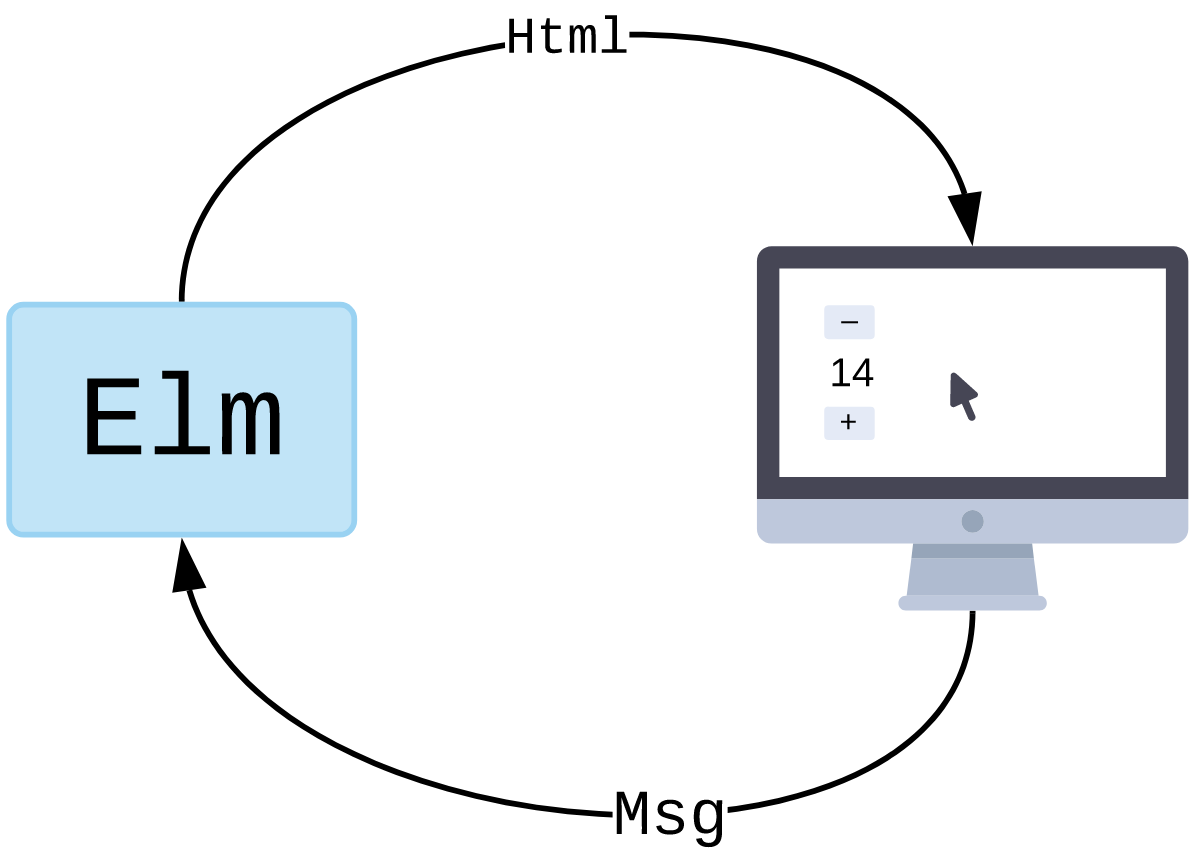
\includegraphics[width=0.5\textwidth]{elm_arch.png}
    \caption{Diagram działania programu w Elmie}\label{fig:elm_arch}
\end{figure}

\textit{The Elm Architecture} jest schematem tworzenia interaktywnych aplikacji internetowych lub gier.
Zgodnie z rysunkiem~\ref{fig:elm_arch} typowa aplikacja Elm działa w następujący sposób:
Program generuje pewien kod HTML, który zostaje wyświetlony na ekranie, a następnie komputer zwraca wiadomości informujące o tym co się dzieje, np.~użytkownik wcisnął guzik.

A co się dzieje wewnątrz wspomnianego programu Elmowego? Zawsze składa się z trzech podstawowych elementów:
\begin{itemize}[noitemsep,topsep=0pt]
    \item Model --- opisujący stan aplikacji
    \item Update --- opisujący logikę aplikacji
    \item View --- opisujący wygląd aplikacji
\end{itemize}

W kolejnych podrozdziałach przedstawiam powyższe elementy architektury Elma na podstawie prostego programu, którego zadaniem jest wyświetlenie na ekranie dwóch guzików oraz licznika, który może się zwiększać i zmniejszać, w zależności od tego, który guzik zostanie naciśnięty przez użytkownika.

\subsection{Model}
\begin{minipage}{.50\textwidth}
    Celem modelu przedstawionego na listingu~\ref{lst:Model} jest zdefiniowanie danych w naszej aplikacji.

    W tym przypadku model będzie bardzo prosty --- jest to rekord zawierający jedną wartość całkowitoliczbową (typ \texttt{Int}), która będzie mogła zostać zwiększona lub zmniejszona poprzez naciśnięcie odpowiedniego guzika.
\end{minipage}\hfill
\begin{minipage}{.43\textwidth}
\begin{lstlisting}[caption={\textit{The Elm Architecture} --- Model},label={lst:Model},language={Elm}]
type alias Model = Int


init : Model
init =
  0
    \end{lstlisting}
\end{minipage}\hfill

\subsection{Update}
\begin{minipage}{.43\textwidth}
    \begin{lstlisting}[caption={\textit{The Elm Architecture} --- Update},label={lst:Update},language={Elm}]
type Msg
  = Increment
  | Decrement


update : Msg -> Model -> Model
update msg model =
  case msg of
    Increment ->
      model + 1

    Decrement ->
      model - 1
    \end{lstlisting}
\end{minipage}\hfill
\begin{minipage}{.50\textwidth}
    Funkcja \texttt{update}, która została przedstawiona na listingu~\ref{lst:Update}, ma za zadanie opisywać jak nasz model będzie się zmieniał w czasie.

    Jako argument przyjmuje nowo zdefiniowany typ \texttt{Msg}, który ma dwa warianty --- \texttt{Increment} i \texttt{Decrement}. Typ zostaje dopasowany i w zależności od otrzymanego wariantu, model zostanie odpowiednio zaktualizowany (zmniejszony lub zwiększony) i zwrócony z funkcji.
\end{minipage}\hfill
\subsection{View}
Funkcja \texttt{view}, która została zaprezentowana na listingu~\ref{lst:View}, jako argument przyjmuje model i zwraca kod HTML\@.
Wykorzystany został tutaj handler \texttt{onClick} z biblioteki \texttt{Html.Events}, który po kliknięciu guzika, do którego został przypisany, generuje odpowiednią wiadomość.
Znak plusa generuje wiadomość \texttt{Increment}, znak minusa \texttt{Decrement}.
Następnie wybrana wiadomość trafia do funkcji \texttt{update}.

\begin{lstlisting}[caption={\textit{The Elm Architecture} --- View},label={lst:View},language={Elm}]
view : Model -> Html Msg
view model =
  div []
    [ button [ onClick Decrement ] [ text "-" ]
    , div [] [ text (String.fromInt model) ]
    , button [ onClick Increment ] [ text "+" ]
    ]
\end{lstlisting}

\section{Narzędzia}
Platforma Elm jest dostarczana wraz z zestawem narzędzi pozwalających m.in.~na kompilację plików źródłowych czy instalację dodatkowych modułów. Poniżej postaram się opisać większość z tych narzędzi, tj.~dostarczanych przez Elma, ale wskazać również te dostarczane przez zewnętrznych twórców, a które znacząco ułatwiły mi pracę z tym językiem.
\begin{center}
    \begin{tabularx}{\textwidth}{clX}
        \texttt{elm repl} &---& otwiera interaktywną sesję programistyczną.\\
        \texttt{elm init} &---& inicjalizuje bieżący katalog jako nowy projekt Elma poprzez stworzenie pliku \texttt{elm.json} opisującego projekt i jego zależności, a także tworzy katalog \texttt{src/}, w którym będą znajdowały się pliki \texttt{.elm}.\\
        \texttt{elm reactor} &---& uruchamia serwer deweloperski, który poprzez przeglądarkę pozwala wybrać dany plik źródłowy, skompilować go i sprawdzić jak wygląda po zbudowaniu.\\
        \texttt{elm make} &---& pozwala na kompilację kodu źródłowego do HTML'a lub JavaScript'u. Jest to najbardziej ogólna forma kompilacji, jaką udostępnia Elm, ale jest to niezwykle przydatne narzędzie, kiedy projekt stanie się zbyt skomplikowany na korzystanie z \texttt{elm reactor.}\\
        \texttt{elm install} &---& pozwala instalować paczki dostępne na stronie \url{package.elm-lang.org}, które udostępniają nowe funkcjonalności, jak np.~obsługa plików JSON czy praca z zapytaniami HTTP.\\
        \makecell{\texttt{elm-format}~\cite{elm-format}} &---& formater kodu~,,upiększający'' kod źródłowy Elm'a zgodnie z oficjalną dokumentacją opisującą styl jego tworzenia\\
        \makecell{\texttt{elm-live}~\cite{elm-live}} &---& podobnie jak \texttt{elm reactor}, uruchamia serwer deweloperski, jednak jest to znacznie bardziej rozbudowane narzędzie, oferujące m.in.~takie funkcjonalności jak kompilowanie Elm'a do JavaScript'u, załączanie go do pliku HTML i wyświetlanie w przeglądarce stworzonej strony\\
    \end{tabularx}
\end{center}

Ponadto, Elm posiada szeroką dokumentację, która w znacznym zakresie została wykorzystana podczas pracy nad niniejszym dokumentem.
Składa się z dwóch głównych części --- oficjalnego poradnika języka oraz technicznego opisu paczek, zarówno tych podstawowych jak i tych stworzonych i udostępnionych przez użytkowników.

Pierwsza część składa się z poradnika, który opisuje m.in.~podstawowe mechanizmy języka, przedstawia przykłady prostych aplikacji wraz z ćwiczeniami pozwalających na rozwijanie swojej znajomości Elma oraz umiejętności tworzenia oprogramowania z jego wykorzystaniem, a także oferuje wskazówki odnośnie dobrych praktyk pisania kodu w tym języku.

Druga część dokumentacji zawiera techniczny opis zarówno tych fundamentalnych modułów języka, niezbędnych do tworzenia aplikacji internetowych, takich jak \texttt{elm/core} i \texttt{elm/browser}, przez te mniej niezbędne, jednakowoż w wielu przypadkach wymagane do spełnienia podstawowych funkcjonalności tworzonego oprogramowania, np.~\texttt{elm/http} i \texttt{elm/json}.

Dokumentacja techniczna zawiera takie informacje, jak ogólne przeznaczenie danej paczki, jakie moduły są w niej zawarte, a także szczegółowy opis funkcji mieszczących się w ramach danego modułu wraz z przykładami ich użycia.

% ---------------------------------------------------------------------------------------------------------------------

\chapter{Implementacja}
W ramach części praktycznej niniejszej pracy stworzona została aplikacja internetowa typu \textit{startpage}, czyli spersonalizowanej strony startowej przeglądarki zawierającej najpotrzebniejsze i najczęściej używane elementy oraz skróty.
W ramach tejże aplikacji postanowiłem zaimplementować następujące funkcjonalności:
\begin{itemize}[noitemsep,topsep=0pt]
    \item Cyfrowy zegar wskazujący aktualny czas w strefie czasowej użytkownika
    \item Aktualna data
    \item Pogoda w Gdańsku przedstawiona w formie krótkiego opisu oraz temperatury w stopniach Celsjusza
    \item Wyszukiwarka Google
    \item Zakładki zawierające odnośniki do wybranych stron internetowych
\end{itemize}

Powyżej wymienione elementy wykorzystują różne mechanizmy języka, dodatkowe biblioteki Elm'a oraz uwzględniają pracę z najpopularniejszymi sposobami przekazywania informacji w aplikacjach internetowych, takich jak przetwarzanie plików JSON, wysyłanie zapytań HTTP oraz praca z plikami.

W poniższych podrozdziałach skupię się na opisie wymienionych wyżej mechanizmów, bazując bezpośrednio na kodzie źródłowym stworzonej aplikacji.
Przejdę przez każdy fragment architektury Elma, tj. \texttt{Model}, \texttt{View} i \texttt{Update}, opisując działanie najważniejszych według mnie fragmentów kodu oraz wyjaśniając decyzje stojące za wyborem danych rozwiązań.

\section{Model}
Na listingu~\ref{lst:impl_model} przedstawiony został zaimplementowany model aplikacji, którego celem jest reprezentacja aktualnego stanu programu, a także pokazane zostają stworzone typy pomocniczne wykorzystane w głównym typie Model.

\begin{lstlisting}[caption={\textit{}Pełen model aplikacji},label={lst:impl_model},language={Elm}]
type alias Model =
    { clockTime : ClockTime
    , weatherStatus : WeatherStatus
    , searchText : String
    , bookmarks : List Bookmark
    }
type alias ClockTime =
    { zone : Time.Zone
    , time : Time.Posix
    }
type WeatherStatus
    = Failure String
    | Loading
    | Success Weather
type alias Weather =
    { description : String
    , temperature : Float
    }
type alias Bookmark =
    { name : String
    , url : String
    }
\end{lstlisting}

W rozdziale powyżej wymienione zostały główne funkcjonalności aplikacji, które bezpośrednio przekładają się na implementację modelu.
Informacje potrzebne do przedstawienia daty i godziny zawarte zostały w zmiennej typu \texttt{ClockTime}, który zawiera w sobie dane wykorzystujące bibliotekę \texttt{elm/time} do określenia strefy czasowej oraz aktualnego czasu, tj.~daty i godziny.

Kolejnym elementem modelu jest zmienna typu \texttt{WeatherStatus}, która może przyjąć jedną z trzech wartości --- \texttt{Failure}, \texttt{Loading} lub \texttt{Success}.
Odpowiada ona za trzymanie informacji o statusie zapytania HTTP do API dostarczanego przez serwis OpenWeather~\cite{openweather}.
Początkowo inicjalizowany jest jako wariant \texttt{Loading}, w przypadku niepowiedzenia zapytania przypisywany jest wariant \texttt{Failure} wraz z tekstem opisującym błąd, w stworzonej aplikacji jest to.~\textit{,,Error: Couldn't retrieve weather data``}.
W przypadku powodzenia typ \texttt{WeatherStatus} przyjmuje wariant \texttt{Success} wraz z otrzymaną pogodą.
Typ pogody \texttt{Weather} zawiera przeparsowane informacje z pliku JSON odebranego z zapytania HTTP, czyli krótki opis słowny pogody oraz aktualna temperatura w Gdańsku.

Następny element o nazwie \texttt{searchText} odpowiada za trzymanie informacji o frazie wpisanej przez użytkownika w dedykowanym polu tekstowym wyszukiwarki, która po wciśnięciu klawisza Enter ma zostać wyszukana w Internecie, wykorzystując do tego wyszukiwarkę Google.

Ostatni zdefiniowany element modelu jest listą elementów typu \texttt{Bookmark}.
Zadaniem elementu \texttt{bookmarks} jest trzymanie informacji o zakładkach zdefiniowanych przez użytkownika w oddzielnym pliku.
Lista przekazywana jest do programu przy pomocy machanizmu flag, co zostanie opisane w kolejnych podrozdziałach.
Typ zakładki składa się z dwóch elementów --- nazwy, która ma zostać wyświetlona na stronie oraz adresu URL, do którego prowadzi kliknięcie hiperlinku.

\begin{lstlisting}[caption={Funkcja inicjalizująca model},label={lst:impl_init},language={Elm}]
init : List Bookmark -> ( Model, Cmd Msg )
init bookmarks =
    ( Model (ClockTime Time.utc (Time.millisToPosix 0)) Loading "" bookmarks
    , Cmd.batch [ Task.perform AdjustTimeZone Time.here, getWeather ]
    )
\end{lstlisting}

Na listingu~\ref{lst:impl_init} przedstawiona została funkcja \texttt{init}, której zadaniem jest wstępne zainicjalizowanie modelu odpowiednimi wartościami.

Przyjmuje jeden argument, którym jest lista zakładek przekazana jako flaga, a zwraca tuplę zawierającą nowy, zainicjalizowany model oraz komendy, jakie mają zostać wykonane przez program.
Inicjalizacja modelu jest trywialna, należy jedynie w odpowiedniej kolejności przekazać wartości dla każdego z elementów. Zegar zostaje wyzerowany, status pogody przymuje wartosć \texttt{Loading}, a zakładki zostają przypisane bezpośrednio z argumentu funkcji.

Następnie należy wskazać wiadomości, które mają zostać przetworzone przez funkcję \texttt{update} i wykonane przez program na początku działania programu.
W przypadku stworzonej aplikacji są to dwie wiadomości --- jedna odpowiedzialna za dostosowanie odpowiedniej strefy czasowej, druga za wysłanie zapytania HTTP w celu odebrania aktualnego stanu pogody.

\section{Update}
Na listingu~\ref{lst:impl_update} znajduje się implementacja typu \texttt{Msg} definiującego rodzaje wiadomości, jakie mogą zostać odebrane i obsłużone przez funkcję \texttt{update}.

\begin{lstlisting}[caption={Implementacja typu \texttt{Msg} i funkcji \texttt{update}},label={lst:impl_update},language={Elm}]
type Msg
    = Tick Time.Posix
    | AdjustTimeZone Time.Zone
    | UpdateWeather
    | GotWeather (Result Http.Error Weather)
    | UpdateField String
    | Search
update : Msg -> Model -> ( Model, Cmd Msg )
update msg model =
  case msg of
    Tick newTime ->
      ( { model | clockTime = ClockTime model.clockTime.zone newTime }
      , Cmd.none )
    AdjustTimeZone newZone ->
      ( { model | clockTime = ClockTime newZone model.clockTime.time }
      , Cmd.none )
    UpdateWeather ->
      ( { model | weatherStatus = Loading }
      , getWeather )
    GotWeather result ->
      case result of
        Ok weather ->
          ( { model | weatherStatus = Success weather }
          , Cmd.none )
        Err _ ->
          ( { model | weatherStatus = Failure "Error: Couldn't retrieve weather data" }
          , Cmd.none )
    UpdateField searchText ->
      ( { model | searchText = searchText }
      , Cmd.none )
    Search ->
      ( model
      , Nav.load ("https://google.com/search?q=" ++ model.searchText) )
\end{lstlisting}

Przedstawiona powyżej funkcja \texttt{update} w przypadku odebrania wiadomości \texttt{UpdateWeather} wykorzystuje pomocniczą funkcję \texttt{getWeather}, przedstawioną na listingu~\ref{lst:impl_weather}, w celu wykonania zapytania HTTP do API usługi OpenWeather, aby odebrać aktualny stan pogody w Gdańsku.
Aby wysłać prawidłowe zapytanie GET do wspomnianego API, potrzebne są dodatkowe dane.
W przypadku stworzonej aplikacji trzymane są one w oddzielnym pliku o nazwie \texttt{Config.elm} i są to:
\begin{itemize}[noitemsep,topsep=0pt]
    \item Prywatny klucz API do OpenWeather
    \item Miasto --- Gdańsk
    \item Jednostki --- Stopnie Celsjusza
\end{itemize}

Do samego wysłania zapytania została użyta biblioteka \texttt{elm/http} i funkcja \texttt{get}, która wymaga adresu URL, na który ma zostać wysłane zapytanie oraz wskazania funkcji dekodującej otrzymaną odpowiedź.
Funkcja dekodująca jest konieczna do wyłuskania potrzebnych informacji ze względu na statyczne typowanie języka Elm.
Program \textit{nie wie} jaki typ ma odebrane zapytanie, więc obowiązkiem programisty jest jego odpowiednie przetworzenie.

W przypadku stworzonej aplikacji jako odpowiedź zapytania GET spodziewanym formatem pliku jest JSON (\texttt{Http.expectJson}), następnie zostaje przekazany typ odebranej wiadomości (\texttt{GotWeather}), a na końcu dekoder (\texttt{weatherDecoder}), użyty do wydobycia konkretnych informacji.
\begin{lstlisting}[mathescape,caption={Implementacja funkcji \texttt{getWeather}},label={lst:impl_weather},language={Elm}]
getWeather : Cmd Msg
getWeather =
  Http.get
    { url = Config.weatherApi ++ ("&q=" ++ Config.city) ++ ("&units=" ++ Config.unit) ++ ("&appid=" ++ Config.apiKey)
    , expect = Http.expectJson GotWeather weatherDecoder
    }
\end{lstlisting}

Do implementacji dekodera użyta została biblioteka \texttt{elm/json}.
Funkcja \texttt{weatherDecoder}, przedstawiona na listingu~\ref{lst:impl_decoder}, ma na celu przetworzenie odebranego pliku w formacie JSON tak, aby pasował do zdefiniowanego przez nas typu \texttt{Weather}, który ma zawierać krótki opis pogody (typ \texttt{String}) oraz temperaturę powietrza (typ \texttt{Float}).

Przykład odpowiedzi w formacie JSON, który na potrzeby prezentacji został zmodyfikowany tak, aby zawierał tylko potrzebne nam informacje, został pokazany na listingu~\ref{lst:impl_json}.
Implementacja funkcji dekodującej wynika bezpośrednio ze struktury odebranej odpowiedzi.
Funkcja \texttt{Json.field} pozwala na wyciągniecie wartości pola o danej nazwie, a \texttt{Json.index} wartości znajdującej się pod wskazanym indeksem.
Na końcu, funkcja \texttt{Json.map2} pozwala na przypisanie wyłuskanych wartości do wskazanego typu, tutaj \texttt{Weather}.

Znając działanie tych funkcji można zauważyć że implementacja funkcji dekodującej jest dość prosta:~,,sprecyzuj typ i miejsce potrzebnych pól z odpowiedzi JSON, a następnie zmapuj je do wskazanego typu``.

\begin{lstlisting}[mathescape,caption={Implementacja dekodera JSON},label={lst:impl_decoder},language={Elm}]
weatherDecoder : Json.Decoder Weather
weatherDecoder =
  Json.map2 Weather
    (Json.field "weather" (Json.index 0 (Json.field "description" Json.string)))
    (Json.field "main" (Json.field "temp" Json.float))
\end{lstlisting}
\begin{lstlisting}[mathescape,caption={Przykład odebranego zapytania GET w formacie JSON},label={lst:impl_json}]
"weather": [ {
    "description": "broken clouds",
  }
],
"main": {
  "temp": 20.58,
}
\end{lstlisting}

Przechodząc do implementacji cyfrowego zegara, do jego prawidłowego działania potrzebne jest wykorzystanie funkcji \texttt{subscriptions}, której zadaniem jest cykliczne generowanie wiadomości typu \texttt{Msg}. Na listingu~\ref{lst:impl_subs} przedstawiona została implementacja tej funkcji dla stworzonej aplikacji. Wykorzystanie biblioteki \texttt{elm/time} pozwala na użycie funkcji \texttt{Time.every} z argumentem \texttt{10}. W praktyce oznacza to, że co 10 \textit{ms} zostanie wygenerowana wiadomość typu \texttt{Tick} wraz z aktualnym czasem POSIX przekazanym jako argument, a następnie funkcja \texttt{update} na podstawie tej wiadomości odpowiednio zaktualizuje wartość \texttt{clockTime.time} w zdefiniowanym modelu.

\begin{lstlisting}[mathescape,caption={Implementacja funkcji \texttt{subscriptions}},label={lst:impl_subs}]
subscriptions : Model -> Sub Msg
subscriptions _ =
    Time.every 10 Tick
\end{lstlisting}

\section{View}
Na listingu~\ref{lst:impl_view} przedstawiona została implementacja głównej funkcji wyświetlającej elementy na ekranie użytkownika --- \texttt{view}.
Dla lepszej czytelności kodu wykorzystuje ona wiele funkcji pomocnicznych.
Każda z nich wyświetla jeden z pięciu elementów funkcjonalnych, które zostały wymienione na początku tego rozdziału.
\begin{lstlisting}[mathescape,caption={Implementacja funkcji \texttt{view}},label={lst:impl_view},language={Elm}]
view : Model -> Browser.Document Msg
view model =
    { title = "Startpage"
    , body =
        [ div [ class "container" ]
            [ viewTime model.clockTime
            , viewDate model.clockTime
            , viewWeather model.weatherStatus
            , viewSearchBar
            , viewBookmarks model.bookmarks
            ]
        ]
    }
\end{lstlisting}

% ---------------------------------------------------------------------------------------------------------------------

\chapter{Instrukcja laboratoryjna}
W poniższym rozdziale przedstawiam przykładową instrukcję laboratoryjną, która krok po kroku przeprowadza czytelnika przez proces tworzenia aplikacji w Elmie, zaczynając od przygotowania środowiska deweloperskiego, przez podstawy języka wraz z ćwiczeniami pozwalającymi na lepsze zrozumienie składni, aż po stworzenie większej aplikacji frontendowej.

\section{Przygotowanie środowiska}
Pierwszą rzeczą, którą należy się zająć przed rozpoczęciem nowego projektu jest przygotowanie odpowiedniego środowiska deweloperskiego.
Należy upewnić się, że wszystkie narzędzia potrzebne do wykonania pracy są zainstalowane i prawidłowo skonfigurowane.
W przypadku pracy z Elm'em będziemy korzystać przede wszystkim z platformy dostarczanej przez autora, edytora tekstu wspierającego podświetlanie składni, a także innych narzędzi wspomagających proces tworzenia oprogramowania z użyciem tej technologii.

\subsection{Platforma Elm}
Najważniejszą rzeczą, jaka będzie nam potrzebna podczas pracy z Elm'em, będzie platforma języka zawierająca m.in.~takie narzędzia jak kompilator oraz menadżer bibliotek.
Poniżej przedstawiam instukcję instalacji tej platformy na systemach operacyjnych Linux i Windows. Po przejściu tych kroków, w wierszu poleceń należy wykonać instrukcję \texttt{elm}.
Jeśli wszystko zostało prawidłowo zainstalowane i skonfigurowane, powinniśmy ujrzeć widok podobny do przedstawionego na rysunku~\ref{fig:elm_output}.
\begin{figure}[H]
    \centering
    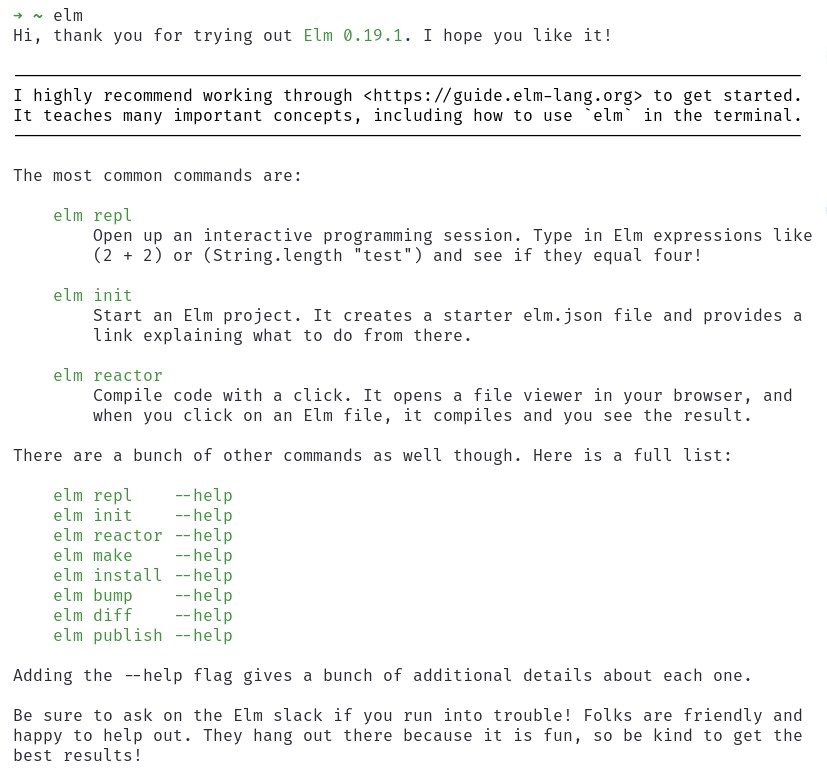
\includegraphics[width=0.95\textwidth]{elm_output.png}
    \caption{Wyjście instrukcji \texttt{elm}}\label{fig:elm_output}
\end{figure}

\subsubsection{Linux}
Najprostszym sposobem instalacji platformy Elm na systemie operacyjnym Linux jest wykorzystanie narzędzia \texttt{npm}~-- powszechnie używanego menadżera pakietów służącego do zarządzania warstwą frontendową aplikacji internetowych.
Aby zainstalować \texttt{npm} należy skorzystać z systemowego menadżera pakietów.
Na przykładzie dystrybucji Ubuntu będą to komendy:
\begin{lstlisting}
  $ sudo apt update
  $ sudo apt install npm
\end{lstlisting}
Kiedy narzędzie zostanie już pomyślnie zainstalowane, można przejść do instalacji platformy Elm.
Posłuży do tego polecenie:
\begin{lstlisting}
  $ npm install -g elm
\end{lstlisting}
Zgodnie z dokumentacją \texttt{npm}~\cite{npmdocs}, flaga \texttt{-g} oznacza, że pakiet zostanie zainstalowany globalnie, dzięki czemu będzie dostępny z każdego miejsca z systemu.
Aby sprawdzić, czy rzeczywiście tak się stało, wystarczy w wierszu poleceń uruchomić komendę \texttt{elm}.
Naszym oczom powinien ukazać się widok podobny do rysunku~\ref{fig:elm_output}, tak jak zostało to już wcześniej wspomniane.
\subsubsection{Windows}
Osoby korzystające z systemu operacyjnego Windows mogą skorzystać z npm, tak jak to było opisane w powyższej sekcji dotyczącej Linuxa lub posłużyć się dedykowanym \href{https://github.com/elm/compiler/releases/download/0.19.1/installer-for-windows.exe}{instalatorem Elm'a}~\cite{elm_installer} na system Windows.
W tym drugim przypadku wystarczy przejść przez wszystkie kroki zostawiając opcje domyślne i w rezultacie Elm zostanie pomyślnie zainstalowany i będzie gotowy do użytkowania.
W celu sprawdzenia czy faktycznie tak się stało, należy uruchomić wiersz poleceń oraz wykonać instrukcję \texttt{elm}. Wyjście komendy powinno być podobne do tego przedstawionego na rysunku~\ref{fig:elm_output}, tak jak zostało to już wcześniej wspomniane.

\subsection{Edytor}
Ważnym elementem tworzenia oprogramowania jest wyposażenie się w odpowiedni edytor tekstowy, który jest w stanie podświetlać składnię języka, z którego aktualnie korzystamy.
Żeby osiągnąć ten cel, w przypadku Elm'a potrzebna będzie instalacja dodatkowej wtyczki do jednego z następujących edytorów:
\begin{itemize}[noitemsep,topsep=0pt]
    \item{\href{https://atom.io/packages/language-elm}{Atom}}
    \item{\href{https://github.com/jcollard/elm-mode}{Emacs}}
    \item{\href{https://github.com/klazuka/intellij-elm}{IntelliJ}}
    \item{\href{https://github.com/rundis/elm-light}{Light Table}}
    \item{\href{https://github.com/evancz/elm-syntax-highlighting/}{Sublime Text}}
    \item{\href{https://github.com/elm-tooling/elm-vim}{Vim}}
    \item{\href{https://github.com/elm-tooling/elm-language-client-vscode}{VS Code}}
\end{itemize}

Powyższa lista zawiera odnośniki do wspomnianych wtyczek dla danego edytora, wystarczy kliknąć nazwę swojego ulubionego edytora i pobrać odpowiedni dodatek.
Na potrzeby niniejszej instrukcji przedstawię proces instalacji i konfiguracji wtyczki dla edytora Visual Studio Code~\cite{vscode}, ponieważ jest to jeden z najbardziej powszechnie używanych narzędzi do pracy z kodem źródłowym.

\subsection{Tworzenie projektu}
Elm jest dostarczany wraz z zestawem bardzo przydatnych narzędzi.
Jednym z nich jest \texttt{elm init}, które posłuży nam do stworzenia nowego projektu.
W tym celu należy otworzyć wiersz poleceń i wykonać następujące instrukcje:
\begin{lstlisting}
  $ mkdir elm_project
  $ cd elm_project
  $ elm init
\end{lstlisting}

Po wypisaniu zawartości katalogu \texttt{elm\_project} z użyciem polecenia \texttt{ls} powinny pojawić się dwa nowe elementy:

\begin{itemize}[noitemsep,topsep=0pt]
    \item{Plik \texttt{elm.json} opisujący projekt oraz jego zależności}
    \item{Katalog \texttt{src/} zawierący nasze przyszłe pliki Elm'a}
\end{itemize}

Następnym krokiem będzie utworzenie nowego pliku \texttt{Main.elm} w nowoutworzonym katalogu \texttt{src/}.
Będzie się tam znajdował kod naszej aplikacji, którą stworzymy w kolejnych krokach.

\section{Podstawy języka Elm}
W celu nauki podstaw języka Elm skorzystamy z narzędzia \texttt{elm repl}, pozwalającego na korzystanie z interaktywnej sesji programistycznej.

\subsection{Wartości}

\subsection{Funkcje}

\section{Aplikacja frontendowa}
W ramach większego projektu zbudujemy stronę internetową typu \texttt{startpage}, czyli strony startowej przeglądarki zawierającej najważniejsze i najczęściej używane elementy.
W naszym przypadku będą to cztery moduły --- zegar, pogoda, wyszukiwarka oraz pasek zakładek.

\subsection{Zegar}

\subsection{Pogoda}

\subsection{Wyszukiwarka}

\subsection{Zakładki}

\subsection{Dokument hipertekstowy}
\begin{lstlisting}[caption={Zawartość pliku \texttt{index.html}},label={lst:index.html},language=html]
<head>
  <link rel="stylesheet" href="assets/styles.css" />
  <script src="assets/main.js"></script>
  <script src="assets/bookmarks.js"></script>
</head>
<body>
  <div id="myapp"></div>
  <script>
    var app = Elm.Main.init({
      node: document.getElementById("myapp"),
      flags: bookmarks,
    });
  </script>
</body>
\end{lstlisting}

\subsection{Style}

% ---------------------------------------------------------------------------------------------------------------------

\chapter{Automatyzacja}
W poniższym rozdziale chciałbym opisać procesy CI/CD oraz korzyści płynące z ich użytkowania, a także zaprezententować implementację takiego rozwiązania na przykładzie stworzonej wcześniej aplikacji w Elm'ie.

\section{CI/CD}
Mianem CI/CD określa się zbiór praktyk pozwających na ciągłą integrację oraz ciągłe wdrażanie projektów informatycznych.
\begin{figure}[H]
    \centering
    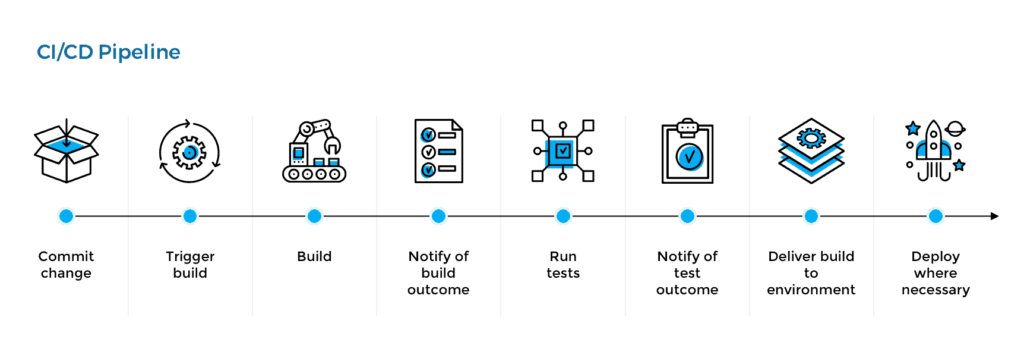
\includegraphics[width=1\textwidth]{cicd_pipeline.png}
    \caption{Przykładowy potok CI/CD}\label{fig:cicd_pipeline}
\end{figure}
Na rysunku~\ref{fig:cicd_pipeline} przedstawiony został przykład potoku CI/CD\@.

\subsection{Ciągła integracja}

Na rynku dostępnych jest wiele narzędzi oferujących usługi wspierające CI\@. Kilka najpopularniejszych z nich to m.in. Jenkins, TeamCity i CircleCI\@.
Są to potężne narzędzia, umożliwiające tworzenie i zarządzanie potokami ciągłej integracji nawet w przypadku bardzo rozbudowanych projektów prowadzonych przez największe firmy informatyczne.
\subsection{Ciągłe wdrażanie}

\section{GitHub Actions}
Od samego rozpoczęcia pracy nad aplikacją w Elmie, cały kod źródłowy przechowywany był z użyciem systemu kontroli wersji Git~\cite{git}, a wybór serwisu hostującego zdalne repozytorium kodu padł na GitHub~\cite{github}. Ze względu na ten wybór jak i niewielki rozmiar stworzonej w Elmie aplikacji, zdecydowałem się wykorzystać GitHub Actions do zbudowania potoków CI/CD\@.


\section{GitHub Pages}
Serwis GitHub udostępnia możliwość hostowania stron internetowych prosto z repozytorium kodu. Warto zaznaczyć, że ta opcja jest dostępna za darmo, pod warunkiem, że hostowana strona znajduje się w \textbf{publicznym} repozytorium kodu. Aby skorzystać z usług GitHub Pages dla prywatnego repozytorium konieczne jest wykupienie jednej z płatnych opcji.

Wykorzystanie funkcjonalności Pages jest dość proste --- w ustawieniach repozytorium należy ustawić gałąź (\textit{branch}), która ma być zbudowana i wystawiona na stronie, a także wybrać odpowiedni katalog.
Domyślnie mogą być to jedynie katalogi \texttt{/} (\texttt{root}) oraz \texttt{/docs}.

Jednakże wykorzystując GitHub Actions możliwe jest bardziej szczegółowe dostosowanie tej strony do swoich potrzeb.
W przypadku stworzonej w ramach tej pracy aplikacji w Elmie, kod źródłowy znajdował się w podkatalogu \texttt{/elm}.
W wyniku stworzonej konfiguracji, na gałęzi \texttt{gh-pages} zostaje opublikowana aktualna zawartość katalogu \texttt{/elm}, a następnie do tej samej gałęzi dodoawany jest otrzymany podczas przeprowadzonej wcześniej fazy budowania wynikowy plik \texttt{main.js}.
GitHub Pages znajduje w wybranym miejscu plik \texttt{index.html}, który zostaje wystawiony i strona staje się dostępna do oglądania.

% ---------------------------------------------------------------------------------------------------------------------

\chapter{Podsumowanie}

\section{Wnioski}

% ---------------------------------------------------------------------------------------------------------------------

\listoffigures
% \listoftables
\lstlistoflistings{}

\printbibliography{}

% ---------------------------------------------------------------------------------------------------------------------

\end{document}
